\chapter{A Dual Chamber Pacemaker Specification}

As part of the model-based design, it is important to have a functional and formal model of the device software for testing and formal verification respectively. In our study, we focus on the implantable  pacemaker since it is one of the simpler implantable cardiac devices as its functionality is based only on timing and does not consider signal morphology. This serves as a good base case to demonstrate the proposed methodology.  In this chapter we describe the basic specification and formal implementation of a dual chamber pacemaker, as well as a more advanced function on mode switching. The specifications are based on the algorithm descriptions in \cite{compass} and the functional description released as part of the Pacemaker Challenge (\cite{challenge}). 
We aim to answer the following questions here:
\begin{itemize}
	\vspace{-5pt}
	\item How are the pacemaker's timers specified to maintain the appropriate heart rhythm?
	\vspace{-5pt}
   	\item What happens if new functionality are applied to the basic model?
\end{itemize}

The artificial pacemaker is designed for patients with bradycardia (i.e. slow heart rate). Two leads, one in the right atrium and one in the right ventricle, are inserted into the heart and fixed onto the inner wall of the heart. These two leads monitors the local activation of the atria and the ventricles, and generate corresponding sensed events (AS, VS) to its software. The software determines the heart condition by measuring time difference between events and delivers pacing events (AP, VP) to the analog circuit when necessary. The analog circuit then delivers pacing signals to the heart to maintain heart rate and A-V synchrony. In order to deal with different heart condition, pacemakers are able to operate in different modes. The modes are labeled using a three character system (e.g. $xyz$). The first position describes the pacing locations, the second location describes the sensing locations, and the third position describes how the pacemaker software responds to sensing. Here we introduce the widely used DDD mode pacemaker which is a dual chamber mode with sensing and pacing in both atrium and ventricle. 

\begin{figure}[!t]
\center
%\vspace{-10pt}
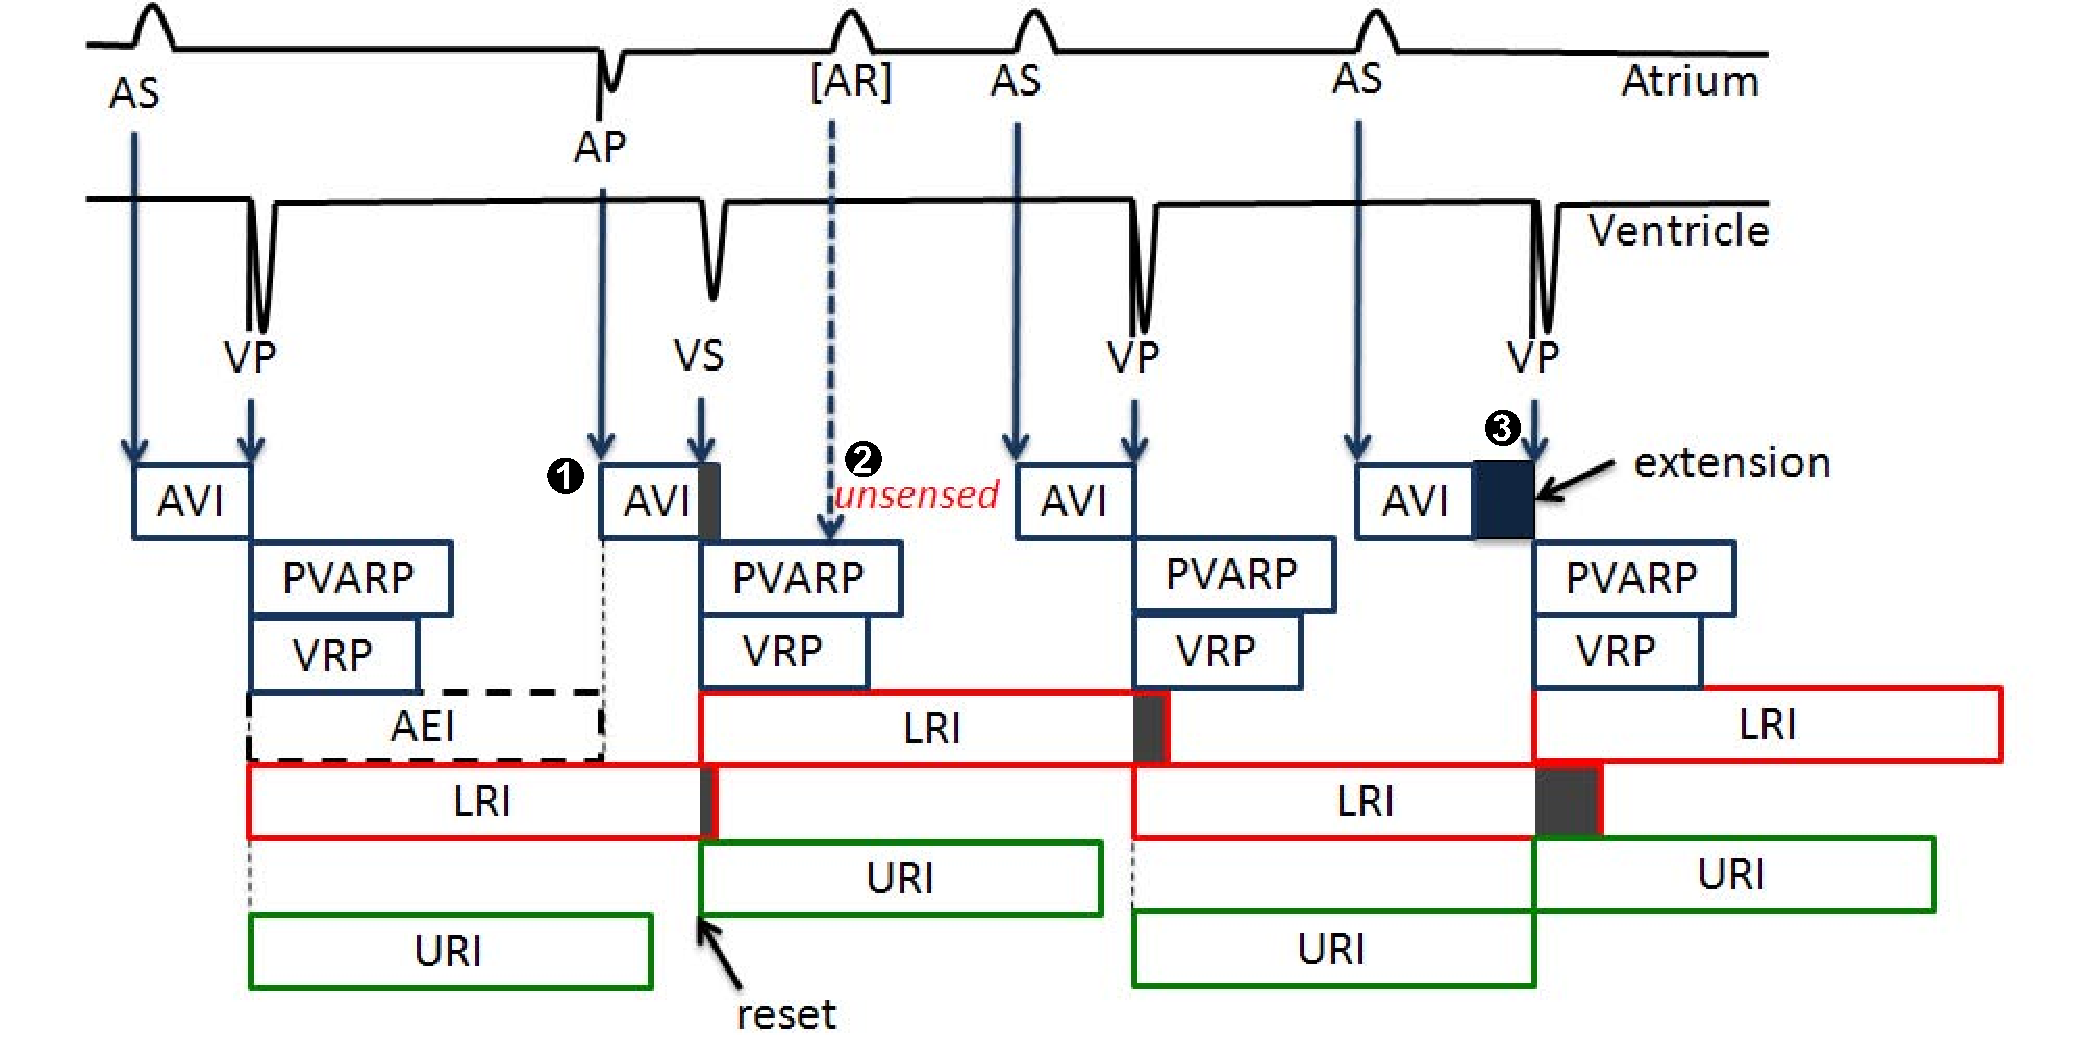
\includegraphics[width=0.7\textwidth]{figs/PM_timers.pdf}
%\vspace{-10pt}
\caption{Basic 5 timing cycles for a dual chamber pacemaker}
\label{fig:PMtimers}
%\vspace{-10pt}t

\end{figure} 
\section{Basic Specifications of a DDD Pacemaker}
The DDD pacemaker has five basic timing cycles triggered by external and internal events, as shown in \figref{PMtimers}. We decomposed our pacemaker model into five components which correspond to the five timers. $P=LRI\| AVI\| URI\| PVARP\| VRP$. These components synchronize with each other using broadcast channels and shared variables (as shown in \figref{PMdesign}). 

\subsection{Lower Rate Interval (LRI)}
%\vspace{-5pt}
The Lower Rate Interval (LRI) component is shown in \figref{PMdesign}(a). This component defines the longest interval allowed between two ventricular events, thus keeping the heart rate above a minimum value. In DDD mode, the LRI interval is divided into a V-A interval (TLRI-TAVI) and a A-V interval (TAVI). The LRI component maintains a maximum V-A delay while the AVI component maintains a maximum A-V delay so together they maintain the maximum V-V delay. In the LRI component, the clock is reset when a ventricular event \textsf{(VS, VP)} is received. If no atrial event has been sensed \textsf{(AS)}, the component will deliver atrial pacing \textsf{(AP)} after TLRI-TAVI. 

%\vspace{-5pt}
\subsection{Atrio-Ventricular Interval (AVI) and Upper Rate Interval (URI)}
%\vspace{-5pt}
The function of the AVI component defines the longest interval between an atrial event and a ventricular event. If there is no ventricular event \textsf{(VS)}  within TAVI after an atrial event \textsf{(AS, AP)}, and the time since the last ventricular event \textsf{(VS, VP)} is longer than TURI, the component will deliver ventricular pacing \textsf{(VP)}. The URI limits the ventricular pacing rate by enforcing a lower bound on the times between consecutive ventricle events. The UPPAAL design of AVI and URI component is shown in \figref{PMdesign}(b) and (c).%The UPPAAL design of AVI component is shown in 

%\vspace{-10pt}
\subsection{Post Ventricular Atrial Refractory Period (PVARP) and Post Ventricular Atrial Blanking (PVAB)}
%\vspace{-5pt}
Ventricular events, especially Ventricular Pace (VP) are sometimes so strong that the atrial lead can sense the activation as well. This signal may be falsely recognized as an atrial event and disrupt normal pacemaker function. This scenario is called crosstalk and was discussed in our previous work (~\cite{vhm_embc11}). In order to prevent this undesired behavior, and filter potential noises, there is a blanking period (PVAB) followed by a refractory period (PVARP) for the atrial events after each ventricular event \textsf{(VS, VP)}. Atrial events during PVAB are ignored and atrial events during PVARP trigger \textsf{AR!} events which can be used in some advanced diagnostic algorithms. The UPPAAL design of PVARP component is shown in \figref{PMdesign}(d).

%\vspace{-10pt}
\subsection{Ventricular Refractory Period (VRP)}
%\vspace{-5pt}
The VRP follows each ventricular event \textsf{(VP, VS)} to filter noise and early events in the ventricular channel which could otherwise cause undesired pacemaker behavior. \figref{PMdesign}(e) shows the UPPAAL design of VRP component.

\begin{figure}[!t]
\center
%\vspace{-10pt}
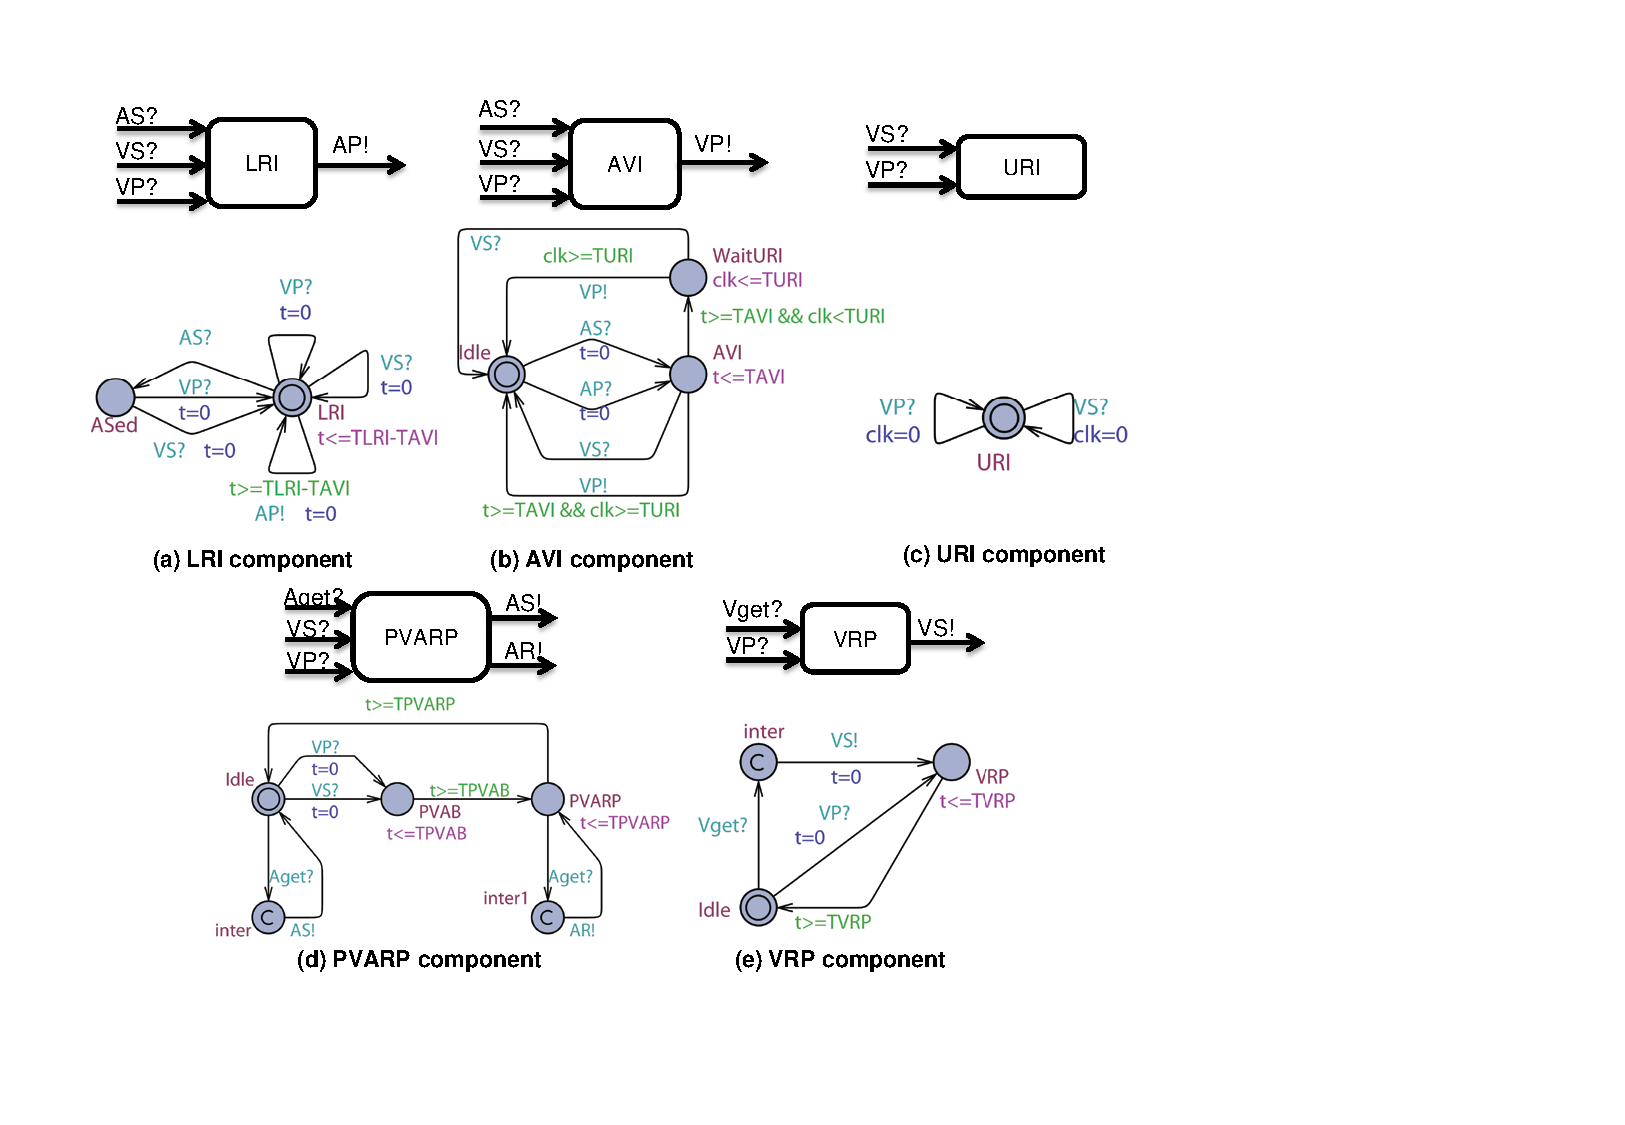
\includegraphics[width=0.9\textwidth]{figs/pacemaker.pdf}
%\vspace{-10pt}
\caption{Basic 5 timing cycles for a dual chamber pacemaker}
\label{fig:PMdesign}
%\vspace{-10pt}
\end{figure} 

\section{Mode Switch Operation: Atrial Tachycardia Response}
Supraventricular Tachycardia (SVT) is an arrhythmia with an abnormally fast atrial rate. %\figref{SVT} is a series of simulation results for closed-loop interaction between a heart model with SVT and the pacemaker model. The atrial and ventricular channels show electrogram inputs to the pacemaker and the pacemaker channel shows the corresponding events received and generated by the pacemaker software, \cite{vhm_embc11}.
Typically, in a heart without pacemaker, the AV node, which has a long refractory period, can filter most of the fast atrial activations during SVT, thus the ventricular rate remains relatively normal. \figref{SVT_none} demonstrates a pacemaker event trace during SVT, with a pacemaker in ODO mode, which just sensing in both channels. 
As there is no pacing in ODO mode, the heart is in open-loop with the pacemaker. In this particular case, every 3 atrial events (AS) correspond to 1 ventricular event (VS) during SVT. 
As an arrhythmia, SVT is still considered a safe heart condition since the ventricles operate under normal rate and still maintain adequate cardiac output. 

However, in the closed loop case with the DDD pacemaker, the AVI component of a dual chamber pacemaker is equivalent to a virtual pathway in parallel to the intrinsic conduction pathway between the atria and the ventricles. The pacemaker tries to maintain 1:1 A-V conduction and thus increases the ventricular rate inappropriately to match the atrial rate.  This is known as Pacemaker Mediated Tachycardia (PMT) as the heart would have been safe without the pacemaker and its virtual pathway. \figref{SVT_DDD} shows the pacemaker trace of the same SVT case with DDD pacemaker. Although half of the fast atrial events are filtered by the PVARP period ([AR]s), the DDD pacemaker still drives the closed-loop system into 2:1 A-V conduction with faster ventricular rate. Maintaining A-V delay is less important than maintaining an appropriate ventricular rate. The DDD pacemaker violates a higher priority requirement in order to satisfy a lower priority requirement, which is inappropriate.
\begin{figure*}[!t]
\centering
		\subfigure [\small]{			
		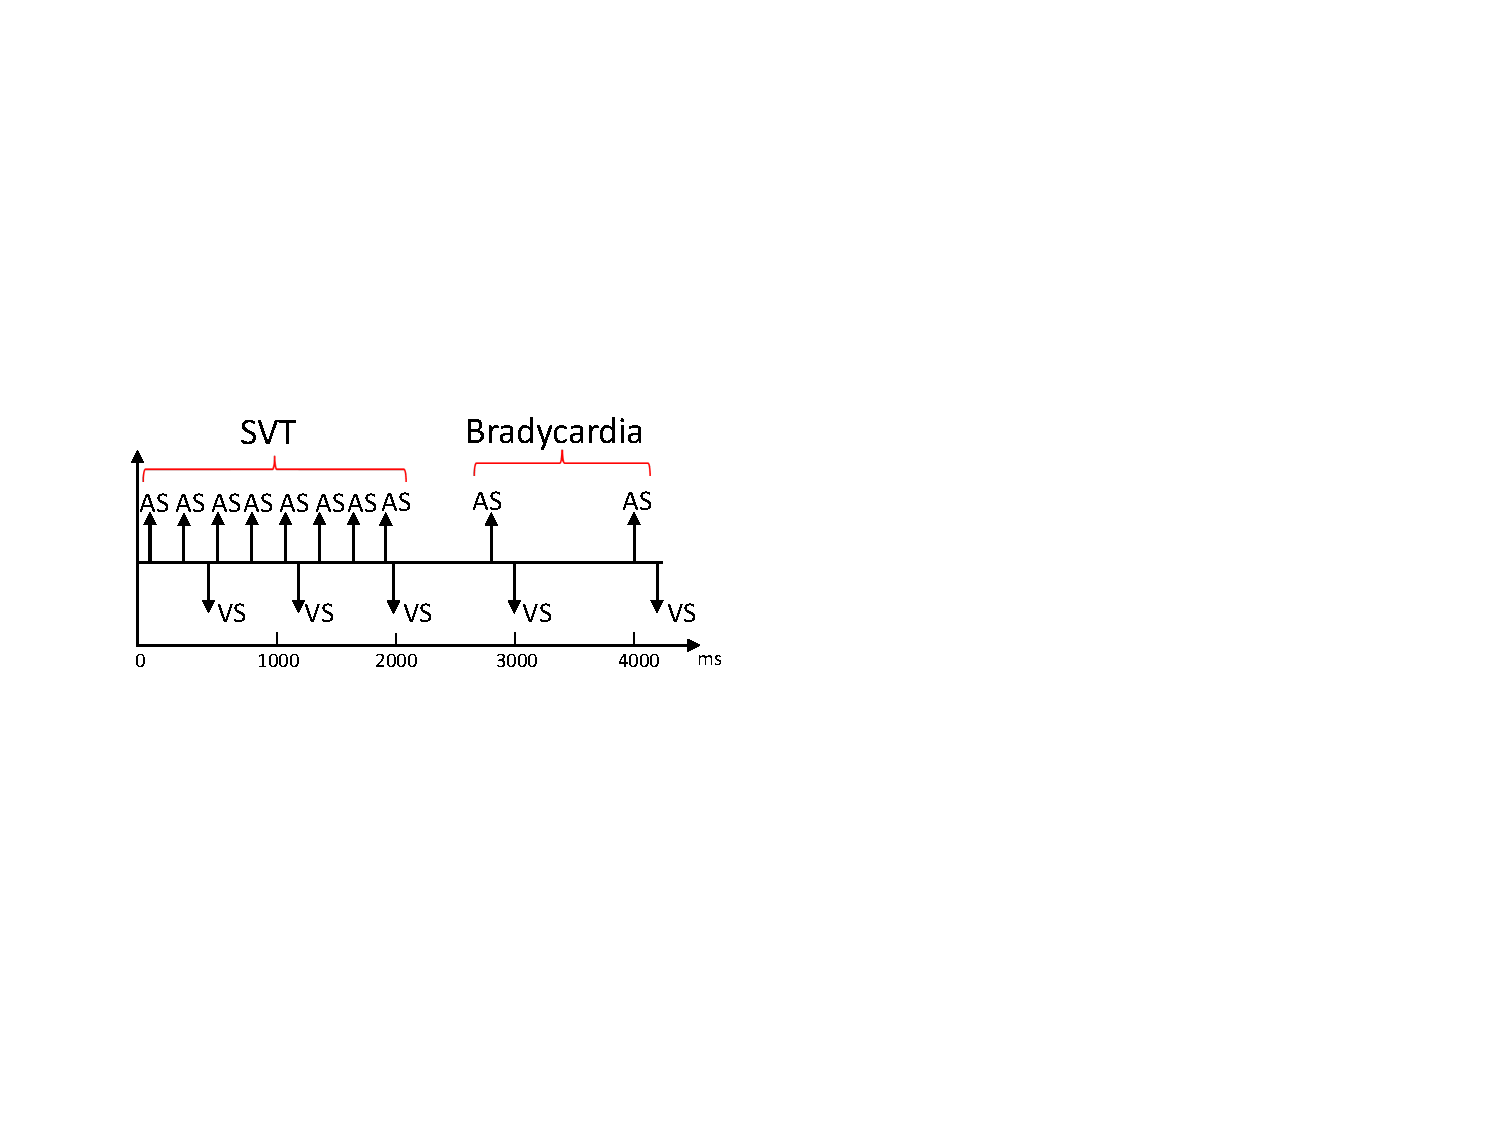
\includegraphics[width=0.5  \textwidth]{figs/SVT_none.pdf}
		\label{fig:SVT_none}
		} 
%	\hspace{.1in}%
\vspace{-10pt}
		
		\subfigure [\small] 
		{
		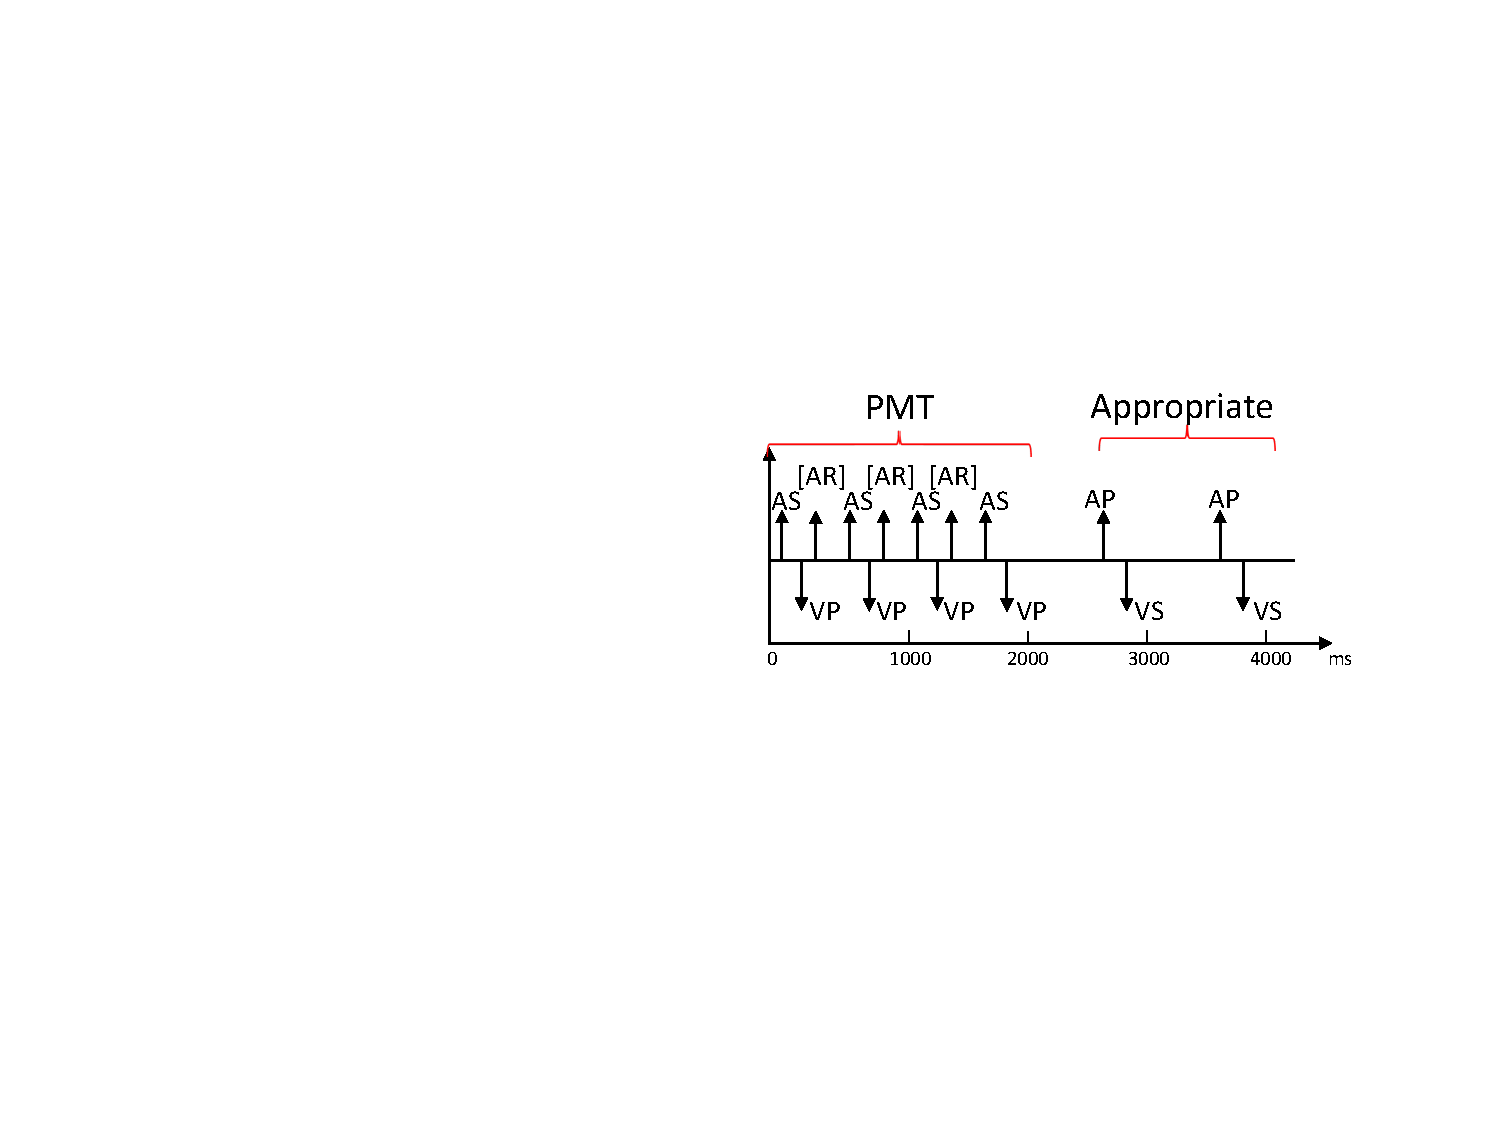
\includegraphics[width=0.5\textwidth]{figs/SVT_DDD.pdf}
		\label{fig:SVT_DDD}
		} 
\vspace{-10pt}
\caption{\small Benign open loop case: SVT with ODO pacemaker (b) Dangerous closed-loop-case SVT with DDD pacemaker}
%\vspace{-15pt}
\end{figure*} 

Pacemaker manufacturers have designed algorithms to detect and terminate these behaviors. Intuitively, the mode-switch algorithm first detects SVT. After confirmed detection, it switches the pacemaker from a dual-chamber mode to a single-chamber mode. During the single-chamber mode, the A-V synchrony function of the pacemaker is deactivated thus the ventricular rate is decoupled from the fast atrial rate. After the algorithm determines the end of SVT, it will switch the pacemaker back to the dual chamber mode. 

The mode-switch algorithm (also known as atrial tachycardia response) specification we use is similar to the one described in the Boston Scientific pacemakers' manual (\cite{compass}). The algorithm first measures the interval between atrial events outside the blanking period (AS, AR). The interval is considered as \emph{fast} if it is above a threshold (\emph{Trigger Rate}) and \emph{slow} otherwise. In our UPPAAL model we model it as $INT$ (see \figref{dur_count} (1)). A counter $CNT$ increments for \emph{fast} events and decrements for \emph{slow} events (see \figref{dur_count} (2)). After the counter value reaches the \emph{Entry Count}, the algorithm will start a \emph{Duration} ($DUR$) ,which is a time interval used to confirm the detection of SVT (see \figref{dur_count} (3)). In the \emph{Duration}, the counter keeps counting. If the counter value is still positive after the \emph{Duration}, the pacemaker will switch to the VDI mode (\emph{Fallback mode}). In the VDI mode, the pacemaker only senses and paces the ventricle. At any time if the counter reaches zero, the \emph{Duration} will terminate and the pacemaker is switched back to DDD mode.
% to show some interesting findings. The basic idea of this simplified model is explained in detail. \\
%\mySubSubSection{UPPAAL model for mode-switch algorithm}
In our UPPAAL model of the mode-switch algorithm, we use nominal parameter values from the clinical setting. We define \emph{trigger rate} at 170bpm (350ms), \emph{entry count} at 8, \emph{duration} for 8 ventricular events and \emph{fallback mode} as VDI. 

In order to model both DDD and VDI modes and the switching between them, we made modifications to the AVI and LRI components.
In each component two copies for both modes are modeled, and switch between each other when switching events (DDD, VDI) are received. During VDI mode, VP is delivered by the LRI component instead of the AVI component. The clock values are shared between both copies in order to preserve essential intervals even after switching. The modified AVI ($AVI'$) and LRI ($LRI'$)components are shown in \figref{avi_ms}. 
\begin{figure*}
		\centering
		%\vspace{-19pt}
		\includegraphics[width=0.8\textwidth]{figs/AVI_ms.pdf}
		%\vspace{-10pt}
		\caption{\small (a) After switching to \textsf{VDI} mode, the new LRI component \textsf{LRI'} maintains a minimum V-V interval; (b) After switching to \textsf{VDI} mode, the new AVI component \textsf{AVI'} keeps track of the time after each atrial events.}
		%  \vspace{-20pt}
		\label{fig:avi_ms}
\end{figure*}
\begin{figure*}
		\centering
				%\vspace{-15pt}
		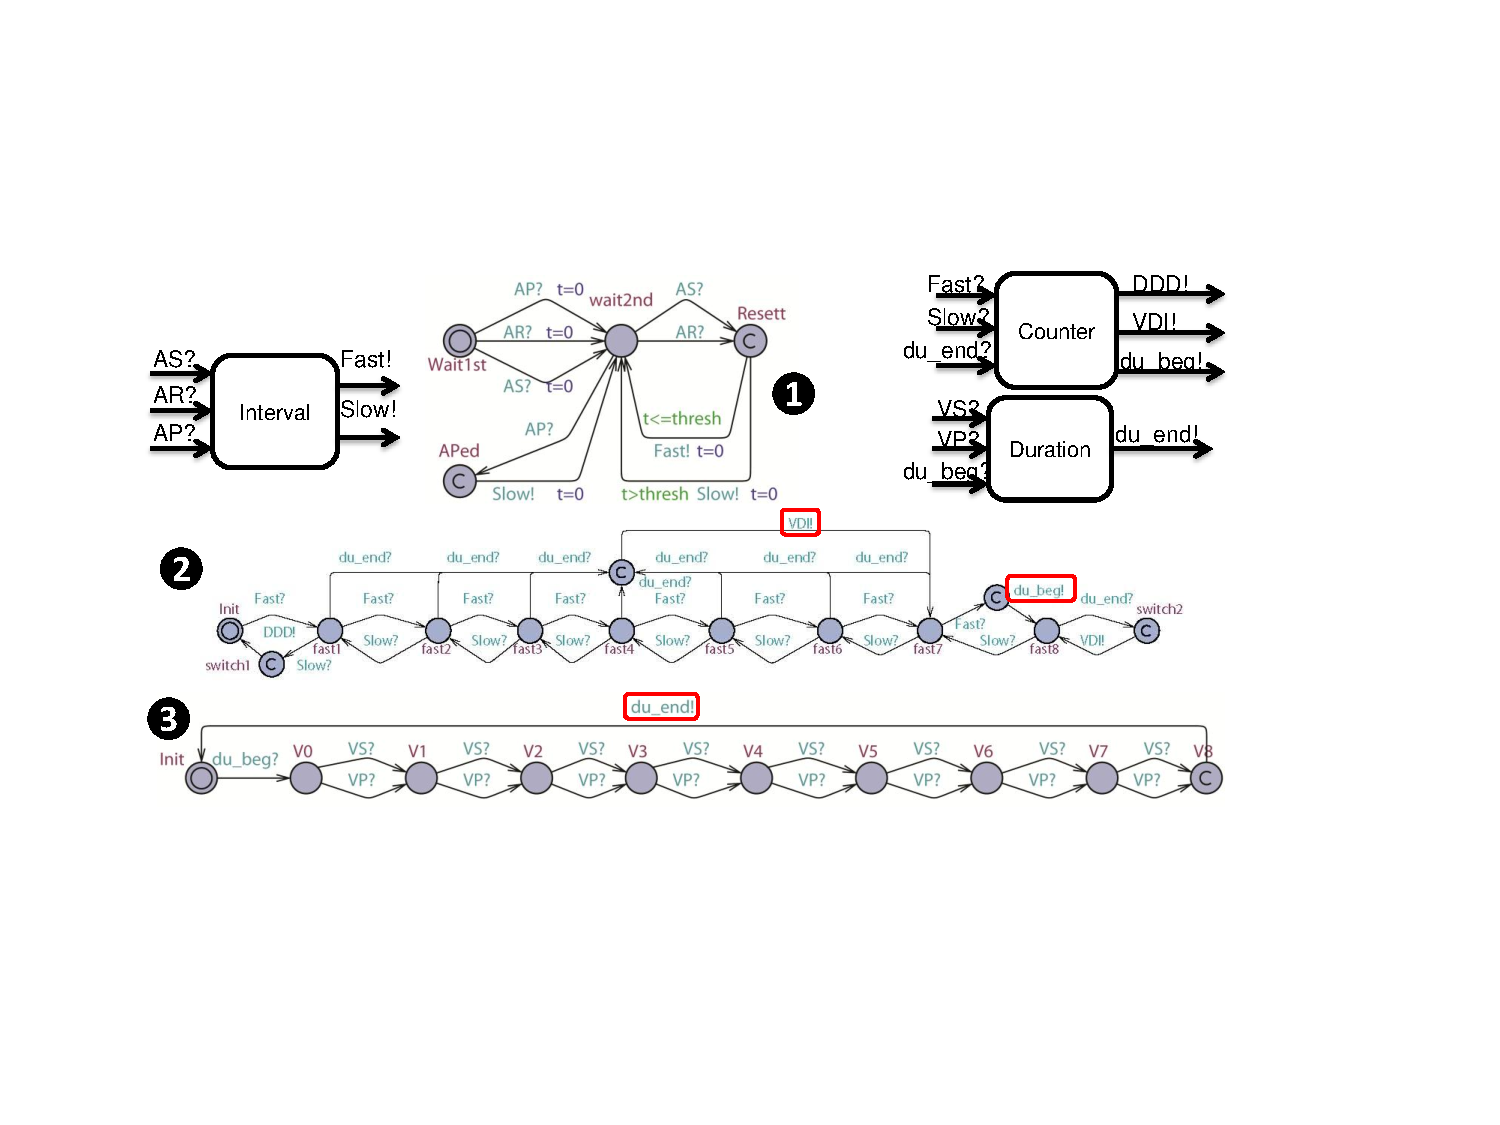
\includegraphics[width=0.9\textwidth]{figs/duration.pdf}
		\vspace{-10pt}
		\caption{\small (1) Component \textsf{INT}: An atrial event (\textsf{AS,AR}) arrives before \textsf{thresh} after the previous atrial event is regarded as a \textsf{fast} event. Atrial event arrives after \textsf{thresh} and \textsf{AP} are regarded as \textsf{slow} event; (2) Component \textsf{CNT}: After 8 \textsf{fast} event the algorithm will start a duration by sending \textsf{du\_beg} and will switch to \textsf{VDI} mode when the duration ends (\textsf{du\_end}); (3) Component \textsf{DUR} :The duration length is 8 ventricular events (\textsf{VS,VP})}
		  %\vspace{-15pt}
		\label{fig:dur_count}
\end{figure*} 

%%%%%%%%%%%%%%%%%%%%%%%%%%%%%%%%%%%%%%%%%%%%
%%%%%%%%%%%%%%%%%%%%%%%%%%%%%%%%%%%%%%%%%%%%

\chapter{Closed-loop Model Checking}
\label{ModelChecking}
There are two categories of device bugs: 
1) the device may fail to conform to its \emph{specifications}, that is, the prescription of how it should react to certain inputs.  
2) the device may fail to improve the conditions of the patient as promised, even if it conforms to its specifications. 
The desired physiological conditions that the closed-loop system should achieve are captured in the \emph{physiological requirements}; for example, for a pacemaker, the heart rate should always be maintained above a certain threshold. 

Bugs in the first category (non-conformance to specification) can be detected via systematic and extensive open-loop testing in which a set of input sequences is fed to the device, and its output is compared with the expected output.
Bugs in the second category (violation of physiological requirements), on the other hand, require the interaction within the \emph{closed-loop system}, which consists of the device and its environment.
For instance, the pacemaker and the heart as its environment. 
In the medical device industry, closed-loop verification of the physiological requirements is mostly performed in terms of clinical trials, in which the actual devices are implanted in human subjects over an extended duration.
Unfortunately, because of the extremely high cost of clinical trials (several million dollars and spanning several years,~\cite{trialcost}), the amount and variety of human subjects during the clinical trials are limited, which reduces the opportunity to find bugs. 
Moreover, clinical trials are often conducted at the final design stage. Fixing bugs at this stage is very costly.

Closed-loop model checking enables closed-loop evaluation of the physiological requirements at an earlier design stage, which requires formal model(s) of the physiological environment. In this chapter we will answer the following questions:
\begin{itemize}	
\vspace{-5pt}
	\item How do model checking results fit into the regulation framework?
	\vspace{-5pt}
	\item How do we find the appropriate abstraction level of the environment model for each physiological requirement?
        \vspace{-5pt}
        \item Exploring the whole state space sounds great. What are the limitations of model checking? 
\end{itemize}
%            \item What are the effects of adding new features to the software? Can they disrupt the safety properties that the previous device hold?

In closed-loop model checking, there is only one device model. 
However there can be a large number of environmental conditions which require different models to represent them. For instance, a heart with atrial flutter has an additional conduction pathway, causing fast atrial rate, that is not present in a healthy heart. The timing and structural differences of different heart conditions should be distinguished in corresponding heart models.
%\todo[inline]{should we give an example of a heart condition?}
A set of initial models of the environment can be constructed, but the set is inherently incomplete because of the large number of environment conditions and their combinations. 
As a result, performing model checking using every model in the set cannot ensure full coverage of the environmental conditions. In the following sections, we will investigate how as we go from basic to more complex requirements, we require more sophisticated approaches to generate and navigate through a variety of environment models. We introduce the concept of an \emph{Abstraction Tree} to systematically encode requirements and choose the appropriate heart models for the requirement. By analyzing the concrete counter-examples we are able to distinguish if the problem is a bug within the device or due to the lack of expressiveness in the environment model. 

%\section{Testing vs Verification}
%
%\newcommand{\ub}{\bar{u}}
%\newcommand{\yb}{\bar{y}}
%
%\emph{\textbf{Testing}} is a method for checking that a system does indeed obey its specification. 
%In testing, an algorithm will do the following:
%\begin{itemize}
	%\item Initialize the system to some initial state $x_0$ in $X_0$.
	%E.g., for a pacemaker device, this would describe the initial values for the various refractory periods, among other things.
	%\item Generate sequences of input strings $\bar{u}_k$ from some set $A$, in reaction to which the system will produce output strings $\bar{y}_k$,
	%\item A \emph{monitor} logs the output strings and determines whether the pair $(\bar{u}_k,\bar{y}_k)$ satisfies the specification or not.	
%\end{itemize}
%
%Because the set of valid initial states $X_0$ and the set of valid input strings $A$ may be infinite (or simply too large), the test bench must decide on how to intelligently choose a \emph{finite} number of $(x_0,\ub)$.
%They must be chosen such that if the system does not produce wrong behavior with these pairs, then it is unlikely to produce errors under the \emph{full} valid set of pairs, namely, $X_0 \times A$.
%This is the main challenge of testing: how to sample an infinite or large set of behaviors such that it is representative (in the above sense) of the full set of behaviors that $S$ is capable of?
%Another important issue in testing is for how long to test the system: i.e. what should be the length of the $k^{th}$ string $\ub_k$? 
%E.g., if $\ub_k$ has length 1000, the bug might manifest itself on $y_1\ldots y_{1001}$, but not $y_1\ldots y_{1000}$.
%
%Regardless of the testing algorithm, testing remains incomplete, in the sense that short of testing every possible behavior, bugs may lie hidden in the behavior that we did not witness.
%
%\emph{\textbf{Verification}} refers to formal verification.
%It is applicable to finite state systems\footnote{Some infinite-state systems can be formally verified after an abstraction process which essentially produces an equivalent system that has finitely many states.}, 
%and requires formal semantics for the system's operation. 
%Roughly, this means we must have a mathematical unambiguous definition of how the system produces its output.
%A verification algorithm, or \emph{model checker}, will explore the \emph{entire finite state-space} of the system in a systematic manner. 
%Intuitively, if the entire state-space has been explored in all possible ways, and no incorrect behavior has been displayed, then the system is correct. 
%Thus, verification is inherently \emph{complete}: if the model checker determines that the system is correct (under the conditions $A$ and $X_0$), then we can rest assured that is indeed the case.
%Unlike testing, there is no question of whether we missed (didn't run) an initial condition that can display a bug.
%There is also no question of test duration.
%However in practice, some bound on the duration of the verification must be placed to avoid excessively long runs. 
%If the model checker can't determine correctness in that time bound, then the verification is inconclusive.
%
%Verification is computationally expensive and usually more burdensome to setup, but comes with a guarantee on the answer. 
%Testing is computationally cheaper and less burdensome to setup, but the guarantees it provides are significantly weaker.
%Testing, on the other hand, may be the only option for some complex systems that are beyond the capacity of today's model checkers, or which do not possess formal semantics.
%
%In this chapter we cover formal verification of the closed-loop system and address testing in the following chapter.
\section{Risk Analysis for Implantable Pacemaker}

\begin{figure}[!t]
		\centering
		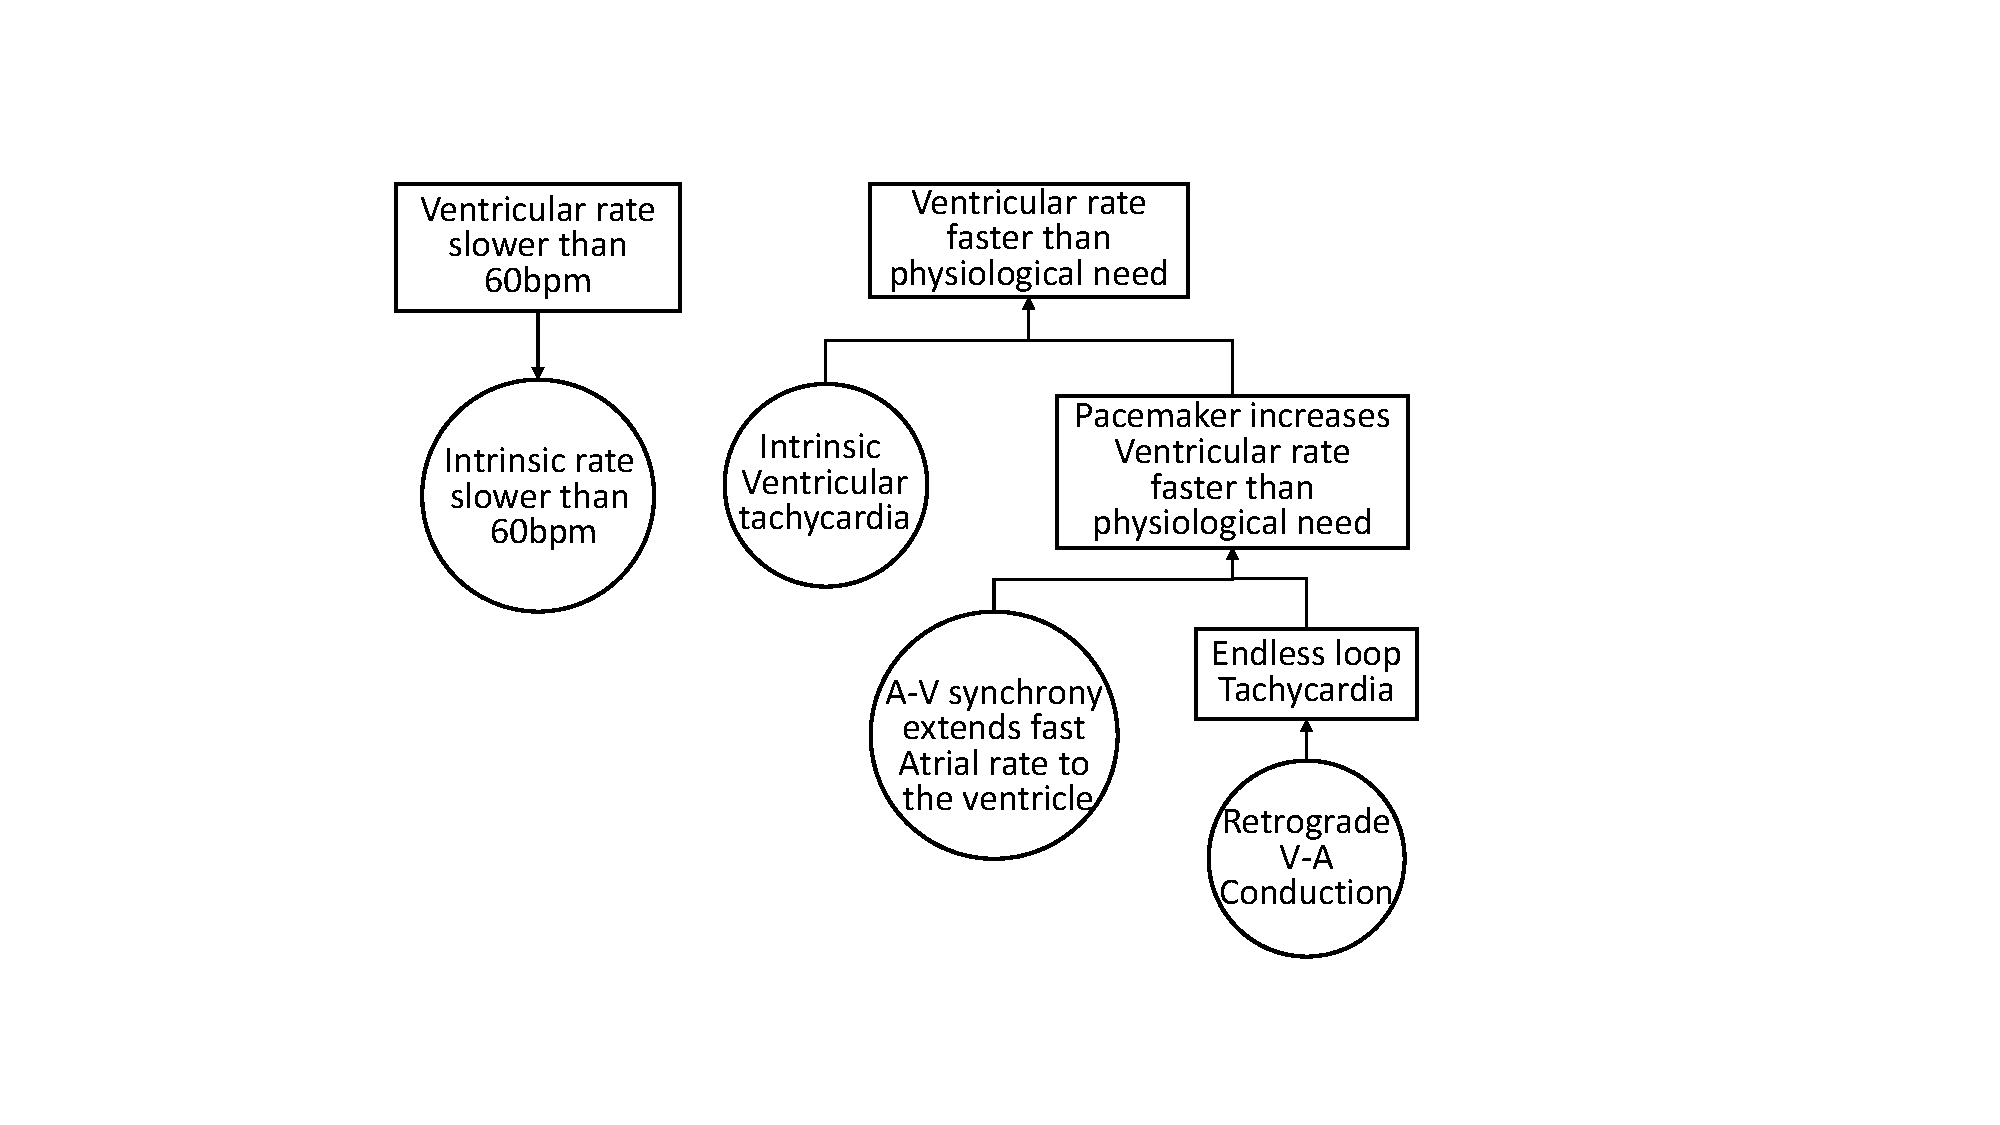
\includegraphics[width=0.9\textwidth]{figs/risk_requirements.pdf}
		\caption{\small }
		  %\vspace{-15pt}
		\label{fig:risk_req}
\end{figure}
\section{Reachability of Unsafe Regions for Basic Pacemaker Function}
The basic function of a pacemaker is to increase heart rate when necessary. As the result, we not only want to verify that the heart rate has been increased accordingly, but also ensure the pacemaker does not increase the heart rate too much. Since these requirements should hold for all possible heart conditions, the most abstract heart model $e$ is selected from Fig. 	\ref{fig:HM_abs} as the environment model. The following two requirements specify the unsafe regions  (too fast and too slow) within the closed-loop state space.

\subsection{Lower Rate Limit}
\vspace{-10pt}
The most essential function for the pacemaker is to treat bradycardia by maintaining the ventricular rate above a certain threshold. We define the region where the ventricular rate is slow, as \textsf{unsafe}. The monitor \textsf{PLRI\_test} is designed to measure intervals between ventricular events and is shown in \figref{safety1}. For property \\
\textsf{$\varphi_{LRI}=$A[] (PLRI\_test.secV imply PLRI\_test.t$\leq$TLRI)}\\ we have $H_4\| P\| PLRI\_test\models\varphi_{LRI}$.

\begin{figure*}[t]
\centering
%\vspace{-10pt}
		\subfigure[Monitor \textsf{PLRI\_test}] {
				\includegraphics[width=0.5\textwidth]{figs/LRI_test.pdf}
				\label{fig:safety1}
		} 
		\subfigure[Monitor \textsf{PURI\_test}] {	
			\includegraphics[width=0.45\textwidth]{figs/uri_test.pdf}
			\label{fig:uri_test}
		}
		%\vspace{-10pt}
	\caption{(a) Monitor for LRL: Interval between two ventricular events should be less than TLRI, (b) Monitor for URL: Interval between a ventricular event and a VP should be longer than TURI}
\vspace{-10pt}
\end{figure*} 

\subsection{Upper Rate Limit}
\vspace{-10pt}
The pacemaker is not designed to treat tachycardia so it can only pace the heart to increase its rate and cannot slow it down. However, it is still important to guarantee it does not pace the ventricles beyond a maximum rate to ensure safe operations. To this effect, an Upper Rate Interval (URI) is specified such that the pacemaker can increase the ventricular rate up to this limit. 

\begin{figure}[b]
		\centering
		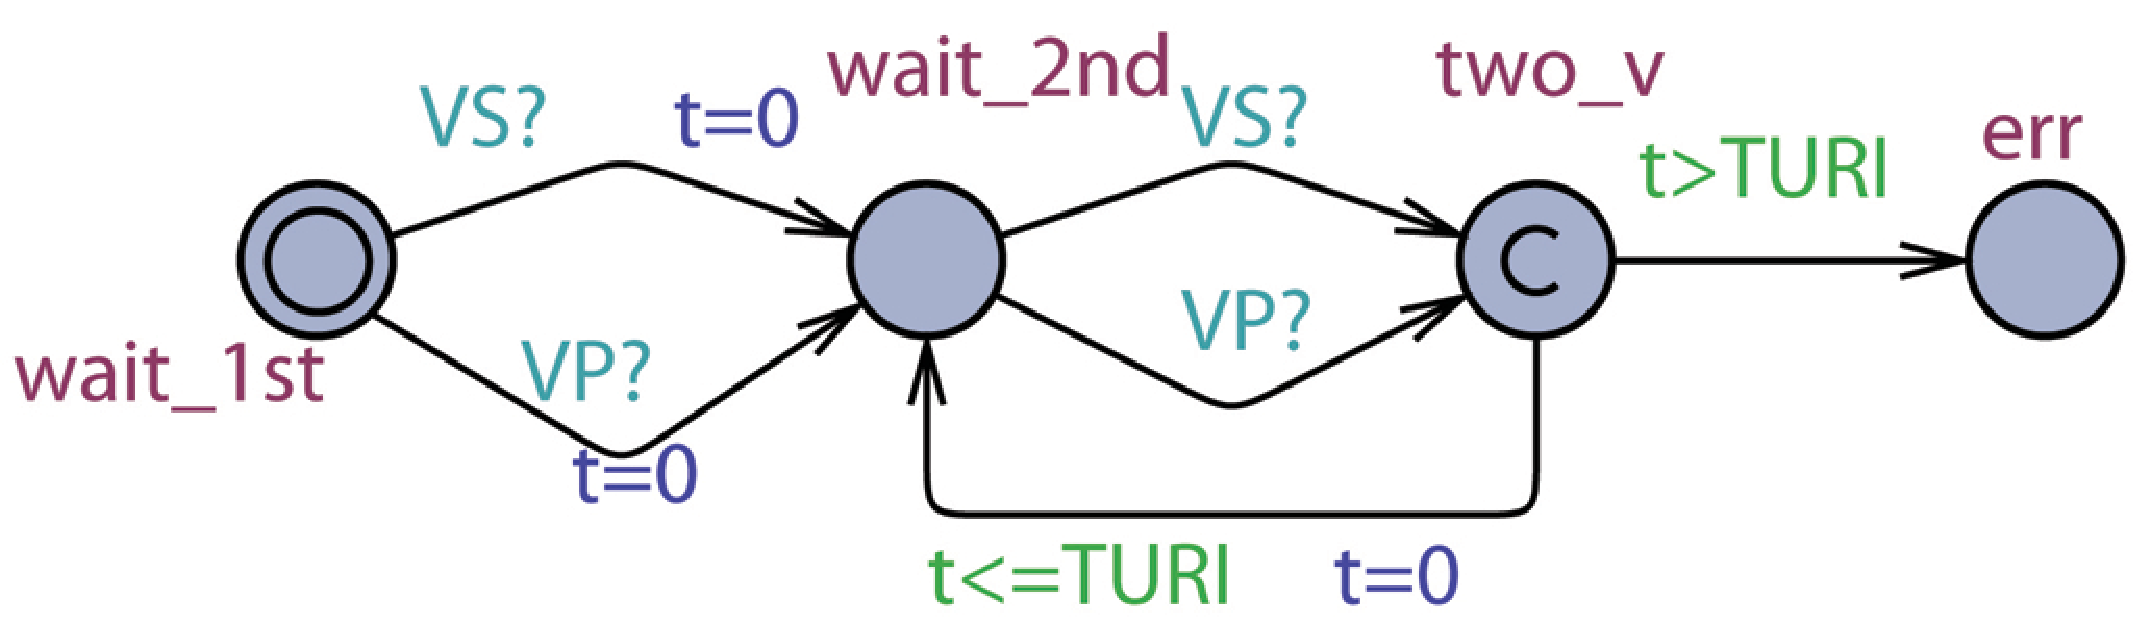
\includegraphics[width=0.4\textwidth]{figs/vv.pdf}
		\caption{\small Monitor \textsf{Pv\_v} for SVT: There exists an endless sequence in which interval between ventricular events is at most TURI}
		  %\vspace{-15pt}
		\label{fig:vv}
\end{figure}
  
We require that a ventricle pace (VP) can only occur at least $TURI$ after a ventricle event (VS, VP). The monitor \textsf{PURI\_test} is shown in \figref{uri_test}. For the property\\
$\varphi_{URI}=$\textsf{A[] (PURI\_test.secV imply PURI\_test.t$\geq$TURI)} \\
we have $H_4\| P\| PURI\_test\models \varphi_{URI}$.

\section{Model Checking the Mode-Switch Algorithm}

\subsection{Existence of Pacemaker Mediated Tachycardia during SVT}
The monitor \textsf{Pv\_v} is designed to show existence of PMT during SVT. It goes to the error state if the ventricular rate drops below the Upper Rate Limit (\figref{vv}).  


We specify 
$\varphi_{MS}=E[] (not Pv\_v.err)$\\
which verifies the existence of PMT. The heart model $H_e$ in Fig. \ref{fig:HM_abs} is not suitable for this property since the non-deterministic conduction of component $P_3$ does not capture the blocking property of the AV node, which is the key in PMT. We use a more refined model $H_d$ which has AV node modeled. To identify the PMT scenario, we first set $H_d.N^1.Trest\_min<100$ so that the atrial rate can be high and $H_d.N^2.Trest\_min>TURI$ so that the intrinsic heart rate is less than TURI. The property is first verified on pacemaker without the mode-switch algorithm. We have $H_d\|P\|Pv\_v\models\varphi_{MS}$ and the evidence returned by the model checker illustrates the PMT scenario.

% There are two separate AVI and LRI components for each mode and switches to the corresponding ones when synchronization signals are received. The clock values are kept so that essential intervals are kept. 
\subsection{Verification against fundamental safety properties}
For a pacemaker with the mode-switch algorithm: $P_2$=\textsf{LRI'$\|$AVI'$\|$URI$\|$PVARP$\|$VRP$\|$INT$\|$CNT$\|$DUR}, we verify the same fundamental safety properties on the pacemaker model with mode-switch algorithm. We have:
$$H_d\|P_2\|PURI\_test\models\varphi_{URI}$$
$$H_d\|P_2\|PLRI\_test\not\models\varphi_{LRI}$$
The Upper Rate Limit property still holds, but the Lower Rate Limit property is violated. The counterexample is proved to be valid after checking the trace of more refined heart models. By analyzing the trace we found that when the pacemaker is switching from VDI mode to DDD mode, the responsibility to deliver VP switched from LRI component to AVI component. Since the clock reference is different (Ventricular events in LRI component and Atrial events in AVI component), the clock value for delivering the next VP is not preserved. As a result, if an atrial event which triggered the mode-switch from VDI to DDD happens within [TLRI-TAVI, TLRI) after the last ventricular event, the next ventricular pacing will be delayed by at most TAVI time, which violates the Lower Rate Limit property (\figref{safety}). 
%%\begin{figure}
%%		\centering
%%		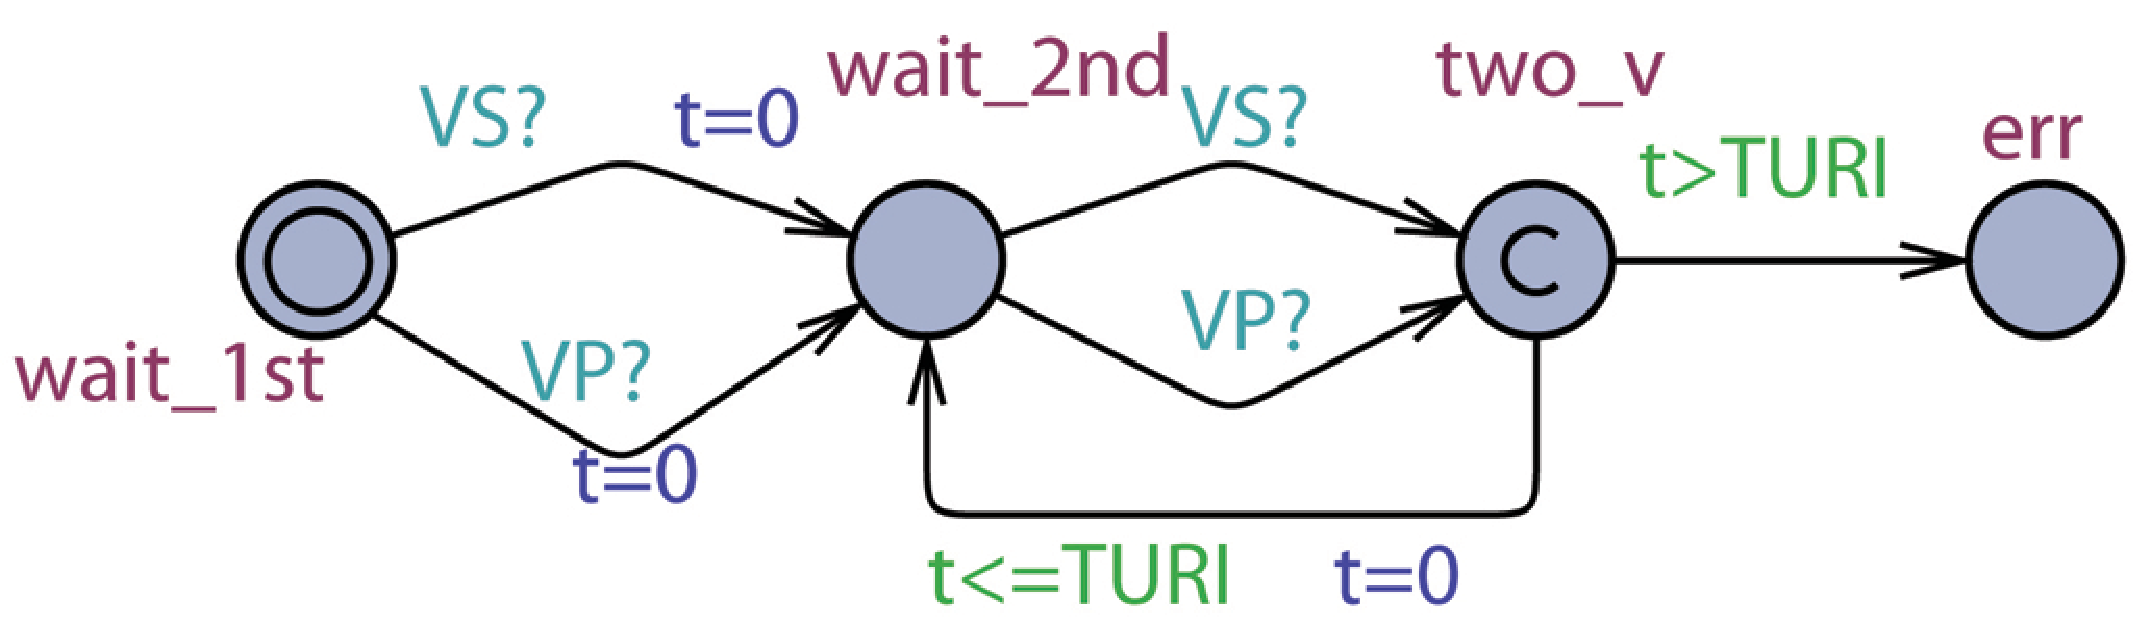
\includegraphics[width=0.4\textwidth]{figs/vv.pdf}
%%		\caption{\small Monitor \textsf{Pv\_v} for SVT: There exists an endless sequence in which interval between ventricular events is at most TURI}
%%		  %\vspace{-15pt}
%%		\label{fig:vv}
%%\end{figure}
\subsection{Verification of the Mode-Switch Algorithm}
After implementing the mode-switch algorithm, we verified the model against the same existence property. We expect the violation of this property, since during VDI mode the ventricular rate of the heart model is less than the Upper Rate Limit and will not trigger ventricular pacing. However, this property is still satisfied, indicating the mode-switch algorithm failed to eliminate the PMT scenario. The evidence trace returned by UPPAAL shows that a subset of atrial events fall into the blanking period after a ventricular event (see \figref{liveness}). As a result, two fast events are reduced to one slow event and mode switch may never happen. This scenario does exist in all our refined heart models, we conclude that the trace is physiologically feasible. The mode-switch algorithm in our pacemaker model can not terminate all PMT behaviors as specified.
\begin{figure}
\centering
%\vspace{-20pt}
		\subfigure []{
				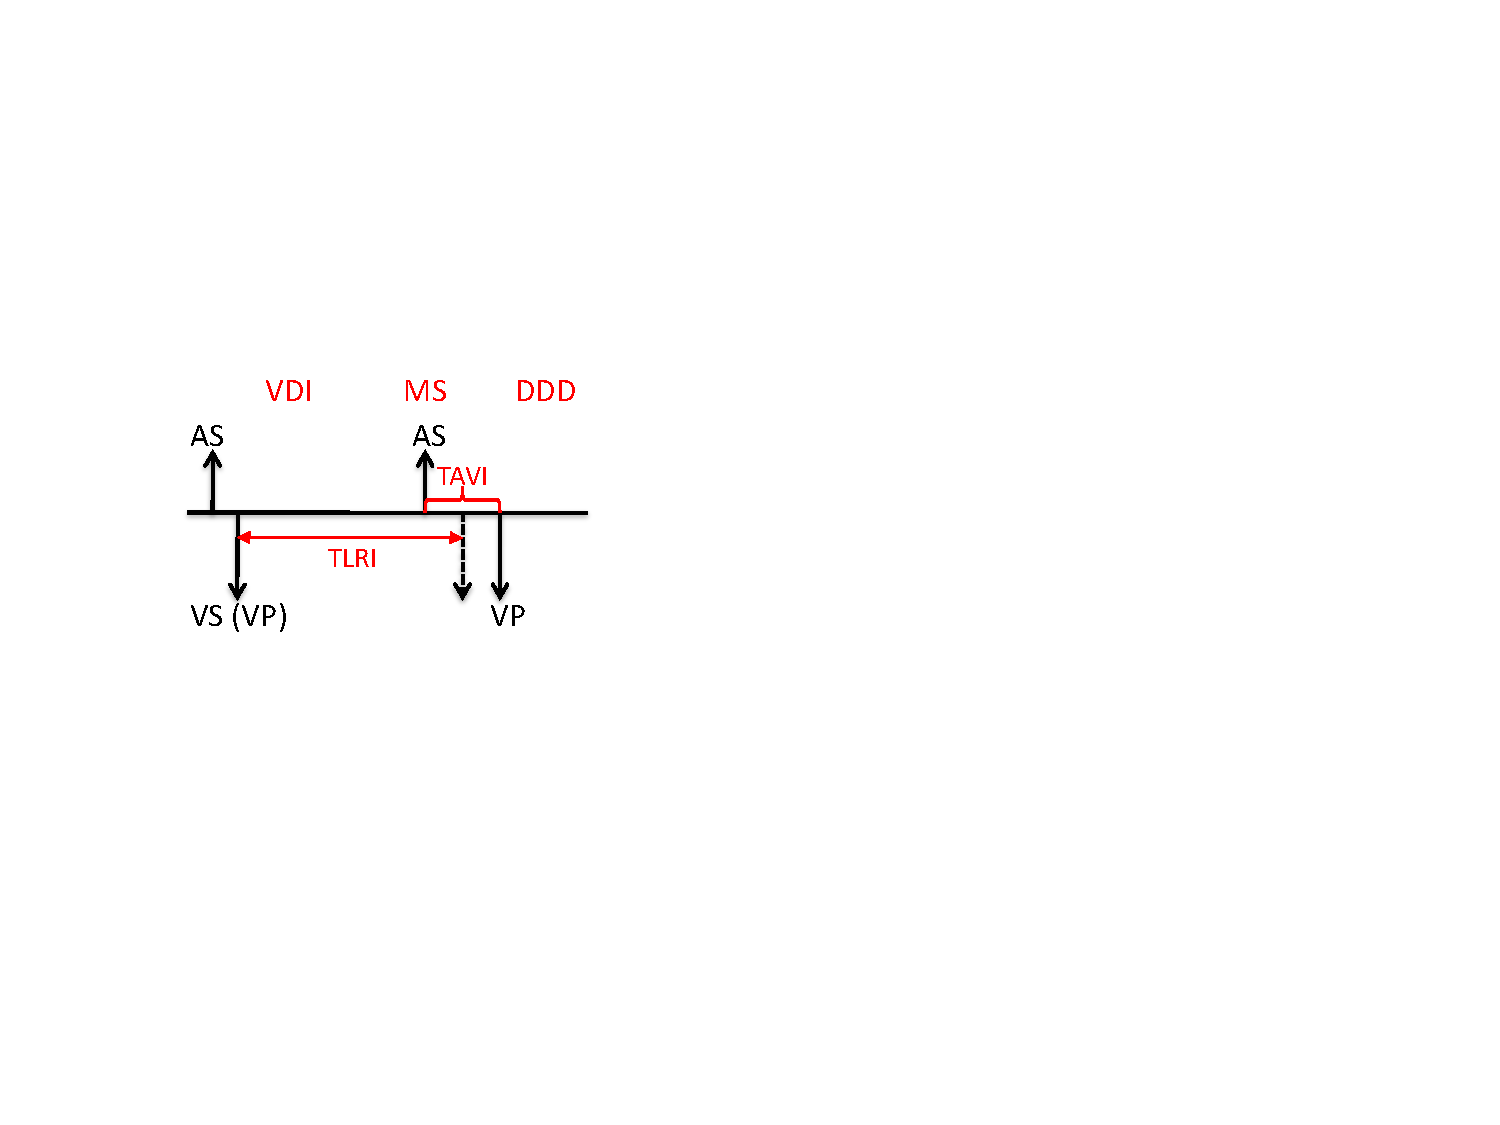
\includegraphics[width=0.4\textwidth]{figs/safety.pdf}
				\label{fig:safety}
		} 
		\subfigure []{	
			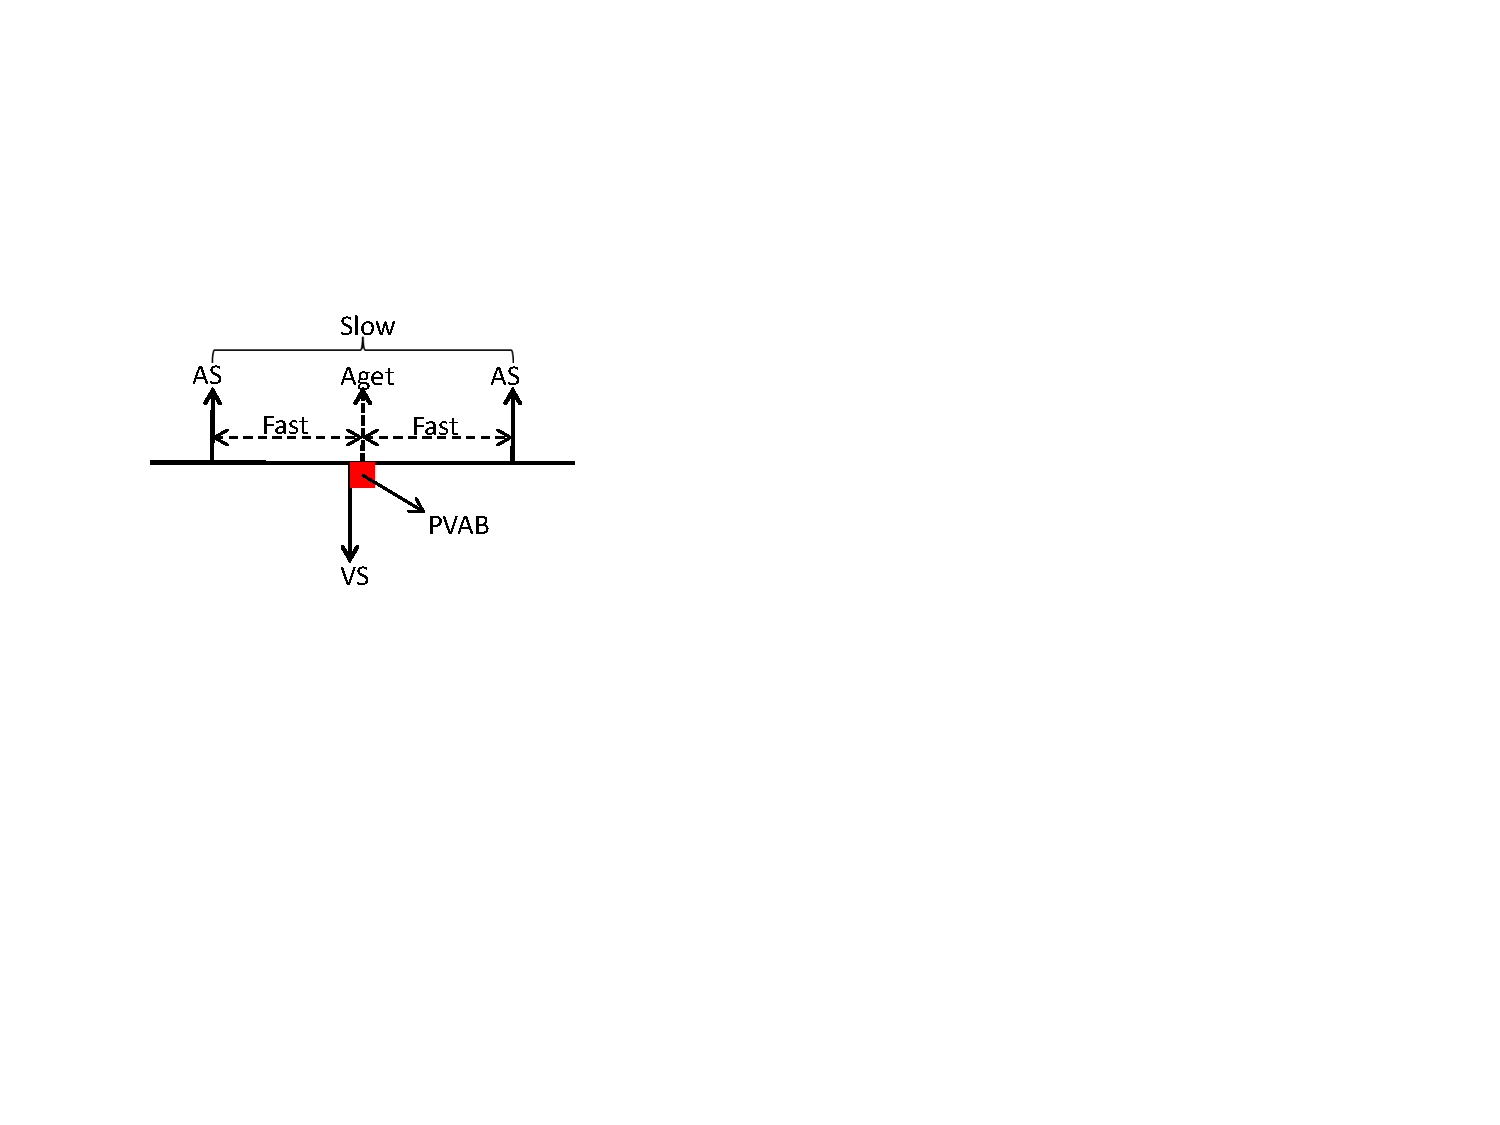
\includegraphics[width=0.4\textwidth]{figs/liveness.pdf}
			\label{fig:liveness}
		}
		\vspace{-10pt}
	\caption{(a) Safety Violation: VP is delayed due to the reset of timer during mode-switch, (b) Correctness Violation: The blocking period may block some atrial events, turning two \emph{Fast} events to one \emph{Slow} event \cite{TACAS12}}
\vspace{-20pt}
\end{figure} 
\section{Abstraction Tree for Environment Modeling}
In the previous two sections, model abstractions and selections are perfomed manually, which require knowledge of both Electrophysiology and model checking. 
Counter-examples returned from abstract models can be difficult to interpret by domain experts.
One abstract counter-example could be produced by multiple physiologically valid conditions, which causes ambiguity.
Thus, a rigorous framework is necessary to balance the need to cover a wide range of environmental conditions and the need to provide counter-examples to the physicians within their physiological context. The framework must also allow non-domain experts to perform verification, and establish `hand-off' points where the results of verification can be handed back 
to the experts for interpretation.

In this section, we use a set of domain-specific abstraction rules developed based on physiological knowledge to ensure the physiological relevance of the behaviors introduced into the abstract models.
The rules are applied to an initial set of physiological models to obtain an abstraction tree, which will be used for closed-loop model checking of the pacemaker. 
A straightforward search procedure is then used to conduct model checking using suitable heart models and return the most concrete and unambiguous counter-examples to the physicians for analysis.
In this framework, physiological knowledge is only needed when constructing the initial model set and when analyzing counter-examples. 
The application of the physiological abstraction rules and the verification procedure can be automated.
The proposed method can potentially be generalized to other domains in which the device operates in a large variety of environmental conditions. More information regarding this research can be found in \cite{regar_tech}.
\subsection*{Step 1: Abstraction Tree Construction}
A set of heart models corresponding to different heart conditions are first developed. 
The list can be expanded as new heart conditions are discovered.
Because we start from a set of initial models, and each one may be abstracted using a number of abstraction rules, we have a choice of which rules to apply to which models, and the order in which to apply them. 
Depending on which rule is applied when, we end up with different abstract models.
Thus an \emph{abstraction tree} $T_{HM}$ for the heart is created, as shown in \figref{HM_tree}. 
%Note that applying rules in different order results different abstraction tree. 
%The order used to obtain $HM\_tree$ is based on the domain knowledge that certain heart conditions may have similar behaviors and similar inputs to the pacemaker. 
%This systematic grouping maintains the physiological-relevance of the heart model even at higher abstraction levels, and reduce the necessity to resolve ambiguities at lower abstraction levels when model checking certain requirements.
\begin{figure}[!t]
	\centering
	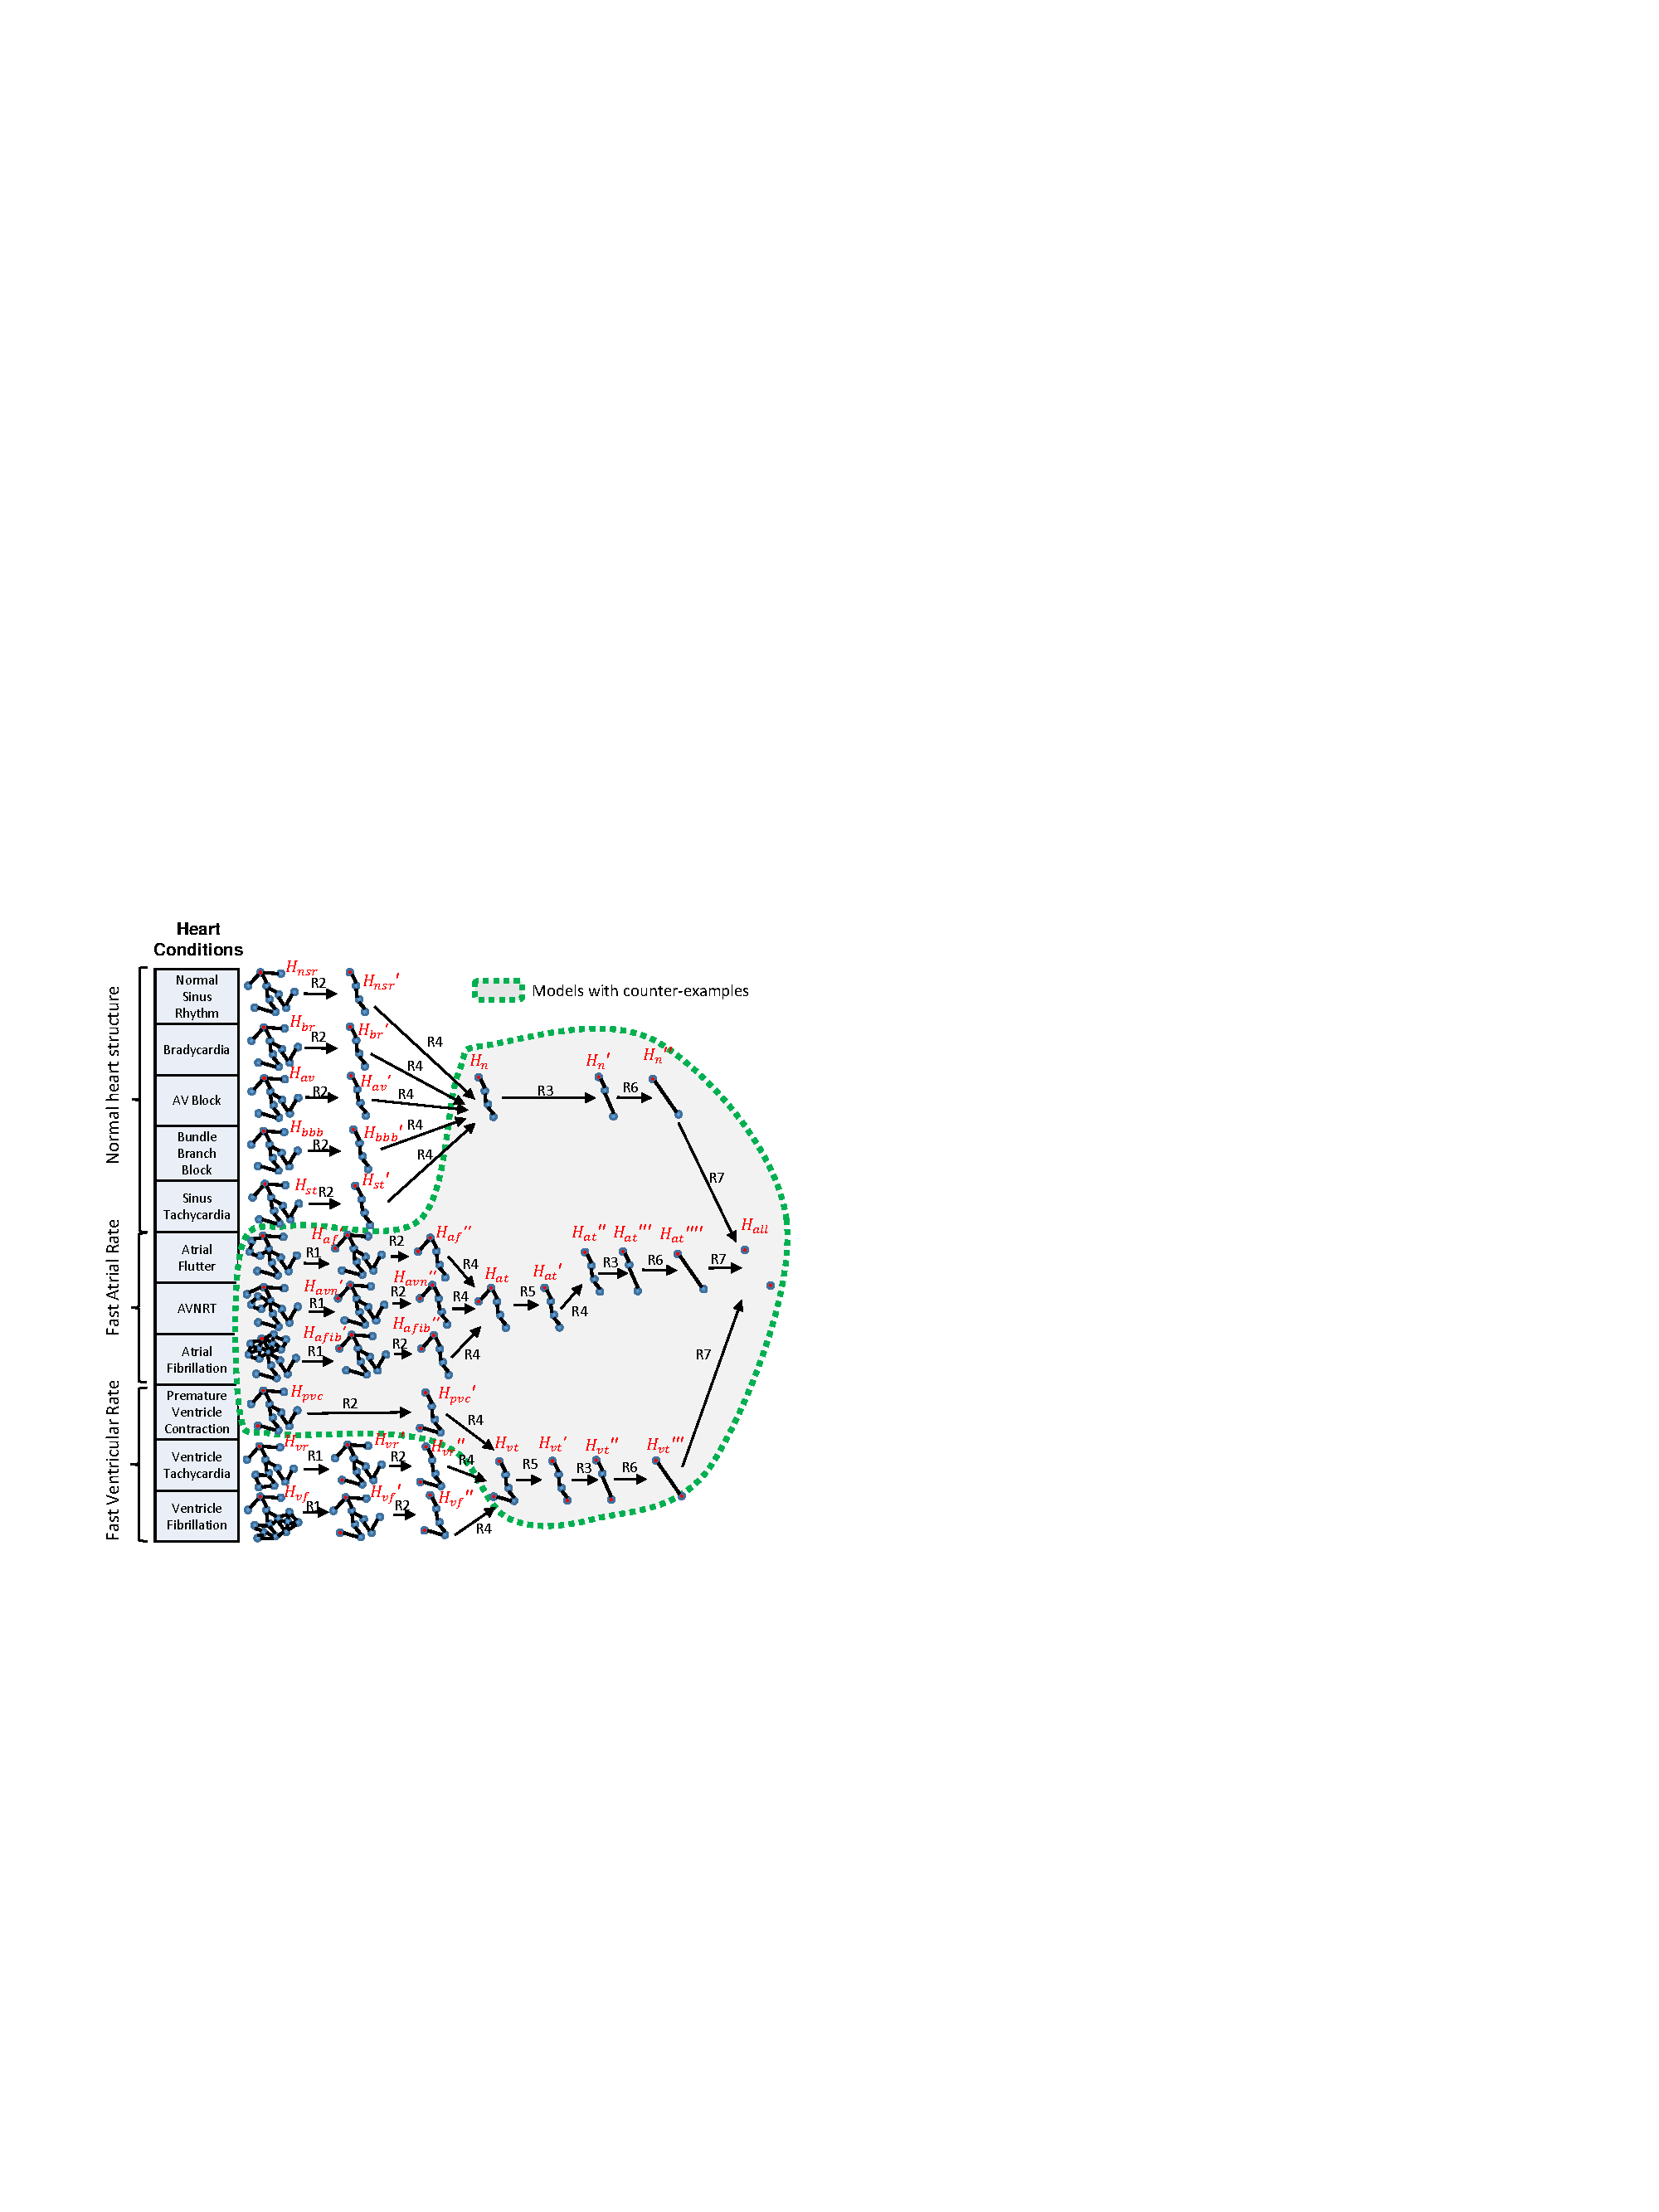
\includegraphics[width=0.85\textwidth]{figs/abs.pdf}
	%\vspace{-5pt}
	\caption{\small Heart Model Abstraction Tree}
	\vspace{-15pt}
	\label{fig:HM_tree}
\end{figure}

\subsection*{Step 2: Requirement Encoding}
The following requirement is designed to prevent the pacemaker from pacing too fast: 
``If the intervals between self-activations of the atria are between 300ms to 1000ms (60bpm - 200bpm), the intervals between ventricular paces should be no shorter than 500ms.''
Self-activation of the atria can be expressed using the location and clock of node automaton $N_A$.
The requirement can be formalized using the monitor  $M_{sing}(VP,500,\infty)$:
%\hatodo{mention $N_A$ is the atrium node automaton}
\[Req1: N_A.loc=Rest \land N_A.t\in [300,1000] \Rightarrow \neg M_{sing}.loc==Err\]
%\todo[inline]{some figure captions are all caps, others are not. please use same thing throughout}
%\begin{figure}[!b]
	%\centering
	%\vspace{-10pt}
	%\includegraphics[width=0.5\textwidth]{figs/abs_sim.pdf}
%
	%\caption{\small Abstraction Rule Application Example}
%\vspace{-10pt}
	%\label{fig:abs_exam}
%\end{figure}
 \subsection*{Step 3: Choosing Appropriate Heart Models For the Requirement}
To verify the closed-loop system with pacemaker model $PM$ and abstraction tree $T_{HM}$ (\figref{HM_tree}) against requirement $Req1$, the most abstract appropriate models are selected from the tree. 
The single event monitor $M_{sing}$ from \figref{monitor}(a) with variables $Var(M_{sing})=\{M_{sing}.t,M_{sing}.loc\}$ is used for this requirement. Model checking is performed on the closed-loop system including the heart model $M_H$, the pacemaker model $M_P$, and the monitor $M$. The requirement $\varphi_P$ can be then represented with TCTL formula:
 \textsf{A[] (not M.Err)}

The variables in the requirement are:
$Var(Req1)=\{N_A.t,N_A.loc,M_{sing}.loc\}$.
\begin{figure}[b]
		\centering
		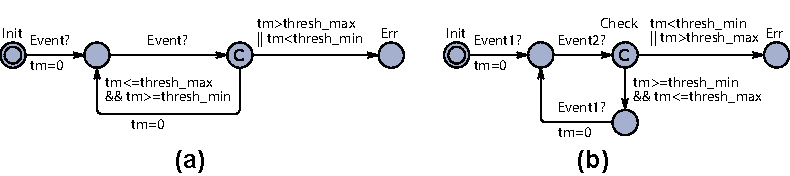
\includegraphics[width=0.8\textwidth]{figs/monitor.pdf}
		%\vspace{-5pt}
		\caption{\small (a) $M_{sing}$ for single event; (b) $M_{doub}$ for two events}
		  \vspace{-10pt}
		\label{fig:monitor}
\end{figure}

At the root of the tree $H_{all}$, we have $\{N_A.t,N_A.loc\} \not \subset Var(H_{all})\cup Var(M_{sing})$. 
So $H_{all}$ is not appropriate for $Req1$. 
All the children of $H_{all}$: $H_n'',H_{at}'''',H_{vt}'''$ are appropriate for $Req1$,
%we have $Var(Req1)\cup Var(M_{sing})\subset Var(H_n'')=Var(H_{at}'''')=Var(H_{vt}''')$, 
thus these three heart models are output as the most abstract models that are appropriate for $Req1$.
\begin{figure}[!t]
	\centering
	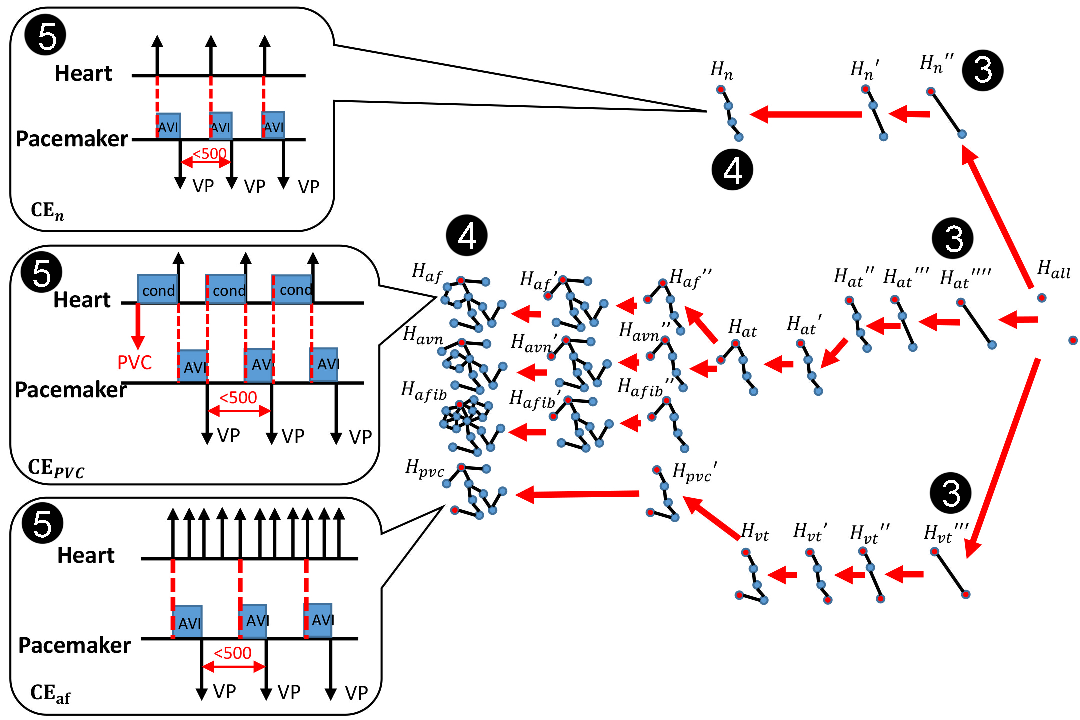
\includegraphics[width=0.8\textwidth]{figs/abs_rev.pdf}
	%\vspace{-5pt}
	\caption{\small Finding the most concrete counter-examples using the abstraction tree}
	\vspace{-10pt}
	\label{fig:CE}
\end{figure}
	\vspace{-10pt}
\subsection*{Step 4: Return the most Concrete Counter-Examples}
After the appropriate models for $Req1$ are selected, we have the initial set
$HM=\{H_n'',H_{at}'''',H_{vt}'''\}$.
Then we run Algorithm 2. By model checking on all 3 initial models in UPPAAL we have: 
$$H_n''||PM\not\models Req1;\; H_{at}''''||PM\not\models Req1;\; H_{vt}'''||PM\not\models Req1$$
%$$[1,[]]=ModelChecking(H_n'',PM,Req1)$$
 %$$[0,CE_1]=ModelChecking(H_{at}'''',PM,Req1)$$
%$$[0,CE_2]=ModelChecking(H_{vt}''',PM,Req1)$$
%\hatodoin{In the following text you use $CE_{at}$, etc. It's  best to use the letter subscripts in the above equations as well, so it's clear which cex comes from which heart model.}
%For the two heart models $H_{at}'''',H_{vt}'''$ in which the requirement is violated, the algorithm keeps going down the abstraction tree, and upon termination counter-examples are returned for the following heart models
The abstraction tree is then further explored. The heart models with counter-examples are illustrated in \figref{CE}, and the most refined heart models with counter-examples are: $H_{n};H_{pvc};H_{af};H_{avn};H_{afib}$.
%$$[0,CE_{at}]=ModelChecking(H_{at},PM,Req1)$$
%$$[0,CE_{pvc}]=ModelChecking(H_{pvc},PM,Req1)$$
%$$[0,CE_{af}]=ModelChecking(H_{af},PM,Req1)$$
%$$[0,CE_{avn}]=ModelChecking(H_{avn},PM,Req1)$$
%$$[0,CE_{afib}]=ModelChecking(H_{afib},PM,Req1)$$

%\begin{figure}[!t]
		%\centering
		%\includegraphics[width=0.9\textwidth]{figs/case.pdf}
		%%\vspace{-5pt}
		%\caption{\small Counter-examples}
		  %\vspace{-10pt}
		%\label{fig:CE}
%\end{figure}
	\vspace{-10pt}
\subsection*{Step 5: Analysis of the Counter-examples}
The counter-examples are then shared with physicians for analysis. In \figref{CE} we highlight three counter-examples. In the first counter-example, the intrinsic heart signals over time with up arrows as atrial activations and down arrows as ventricular activations. The signal for the second counter-example shows the pacemaker outputs with up arrows as atrial pacing and down arrows as ventricular pacing.%We only show the activations of the atrial node and ventricle pacing. 

Counter-example $CE_{n}$ is returned by $H_n$ and none of its children models violate the requirement. By careful analysis we found that $CE_{n}$ features the combination of fast intrinsic atrial rate and prolonged A-V conduction delay, which is the combination of heart conditions $H_{st}$ and $H_{av}$. This scenario shows that the abstraction rules can introduce physiological heart conditions that were not explicitly modeled in the initial model set. The pacemaker improved the open-loop heart condition by pacing the ventricles $AVI$ after each atrial event, which is a correct operation of the pacemaker despite the requirement violation. 
%\hatodo{is it TAVI or AVI like in the previous seciton?}

%\hatodoin{Do you mean that $CE_{at}$ is not a bug? Does this mean that the requirement may be violated in ways that are not dangerous?}
Counter-example $CE_{pvc}$ has a very similar execution to $CE_{n}$. However, the activations of the atrial node are triggered by retrograde conduction from ventricular paces (marker \textsf{cond}). The atrial activations trigger another ventricular pace after $AVI$, which will trigger another retrograde conduction. In this case, the heart rate is inappropriately high, which corresponds to a dangerous closed-loop behavior referred to as \emph{Endless Loop Tachycardia}.

In counter-example $CE_{af}$, the atrial rate is very high, which is also a sub-optimal but not dangerous heart condition. 
However, the ventricular rate can stay normal due to the blocking property of the AV node. 
Despite the filters in the pacemaker, the pacemaker still paces the ventricle for every 3 atrial activations, which extends fast atrial rate to more dangerous fast ventricular rate. 
%\hatodoin{Not very clear..do you mean that the intrinsoc centricular rate is fine because of AV filtering, but the PM is accelarating it?}
This scenario is referred to as Atrial Tachycardia Response of a pacemaker. 

From the analysis, pacemaker operations in $CE_{pvc}$ and $CE_{af}$ must be revised. However, the revision should not affect the behavior in $CE_{n}$. This example demonstrates that counter-examples from refined models provide more physiological context of the requirement violations, and distinguish the physiological conditions that can trigger the violations. The information is helpful for debugging and improving the algorithm. The physicians can also improve the physiological requirement so that these heart conditions can be then considered case by case.
